\usetikzlibrary{math}

\scalebox{0.4}{%
    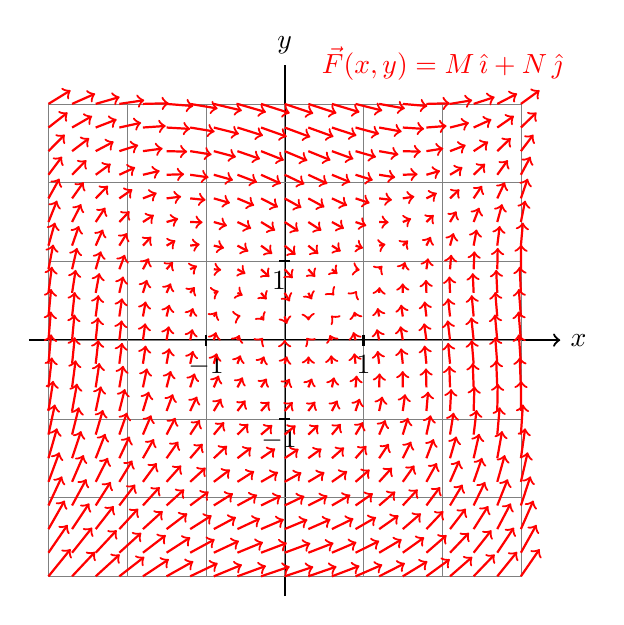
\begin{tikzpicture}
        % Components of the vector field
        \tikzmath{function equis(\x,\y) {return (\y*\y-0.25*\x);};}
        \tikzmath{function ye(\x,\y) {return \x*\x-\y;};}
        \tikzmath{function zeta(\x,\y) {return \x+\y;};}	
        \tikzmath{function magnitud(\x,\y) {return sqrt(\x*\x+\y*\y);};} % magnitude of the vector at (x, y, z)	
        %	
        \pgfmathsetmacro{\dominio}{3.0}	% domain for computation 
        \pgfmathsetmacro{\step}{\dominio/10.0} % step size
        \pgfmathsetmacro{\max}{\dominio}
        \pgfmathsetmacro{\xi}{-\dominio}
        \pgfmathsetmacro{\xf}{\dominio}
        \pgfmathsetmacro{\xs}{\xi+\step}
        \pgfmathsetmacro{\yi}{-\dominio}
        \pgfmathsetmacro{\yf}{\dominio}
        \pgfmathsetmacro{\ys}{\yi+\step}
        % length of coordinate axis
        \pgfmathsetmacro{\ejex}{\dominio+0.50}
        \pgfmathsetmacro{\ejez}{\dominio+0.50}
        % Coordinate axis
        \draw[thick,->] (\xi-0.25,0) -- (\xf+0.5,0) node[right] {$x$}; % Eje x
        \draw[thick] (0,\yi-0.25,0) -- (0,\yf+0.5) node[above] {$y$}; % Eje y
        \draw[help lines] (\xi,\yi) grid (\xf,\yf);
        \foreach \x in {-1,1}
            \draw[thick] (\x,2pt) -- (\x,-2pt) node [below] {$\x$};
        \foreach \y in {-1,1}
            \draw[thick] (2pt,\y) -- (-2pt,\y) node [below] {$\y$};
        % The vector field
        \foreach \x in {\xi,\xs,...,\xf}{
            \foreach \y in {\yi,\ys,...,\yf}{
                % Components of the vector at (\x,\y)
                \pgfmathsetmacro{\vx}{0.125*equis(\x,\y)/(magnitud(\x,\y)+0.1)}
                \pgfmathsetmacro{\vy}{0.125*ye(\x,\y)/(magnitud(\x,\y)+0.1)}
                \draw[red,thick,->] (\x,\y) -- (\x+\vx,\y+\vy);
            }
        }
        \node[red,above,shift={(-1,5pt)}] at (\xf,\yf) {$\vec{F}(x,y) = M\,\hat{\imath} + N\,\hat{\jmath}$};
        %
    \end{tikzpicture}
}